\chapter{Argus}
\label{ch:argus}

Within this chapter, we present Argus\footnote{Inspired by the \textit{all-seeing} giant of the same name from Greek mythology: ``With his multiple sets of eyes, Argus could see nearly everything in his vicinity''. See \url{http://www.loggia.com/myth/argus.html}.}, a partial implementation of our metamodel. We discuss the overall design of Argus and how this fits into the workflow (as presented in \cref{sec:dataset:process}). Additionally, we briefly discuss productivity and performance statistics gathered during the data gathering process, and assess Argus against other comparative tools. Further information related to Argus can be found at \url{http://deakin.edu.au/~ca/argus}, and the source code for Argus is located at \url{http://github.com/alexcu/argus}.

\section{Design}

Argus is designed as a full-screen application to utilise maximum screen space. The application is designed to be keyboard-driven, so shortcuts are displayed wherever possible. Additionally, the current instruction of the workflow is indicated on the top of the image in red to stand out to image taggers. \cref{fig:dataset:argus:overview} shows the main \gls{ui}. Further segment-level features are captured in dialogs or user interaction directly on the image, as shown in \cref{fig:dataset:argus:bib_and_face,fig:dataset:argus:prom_and_col}.

\begin{figure}[h]
  \centering
  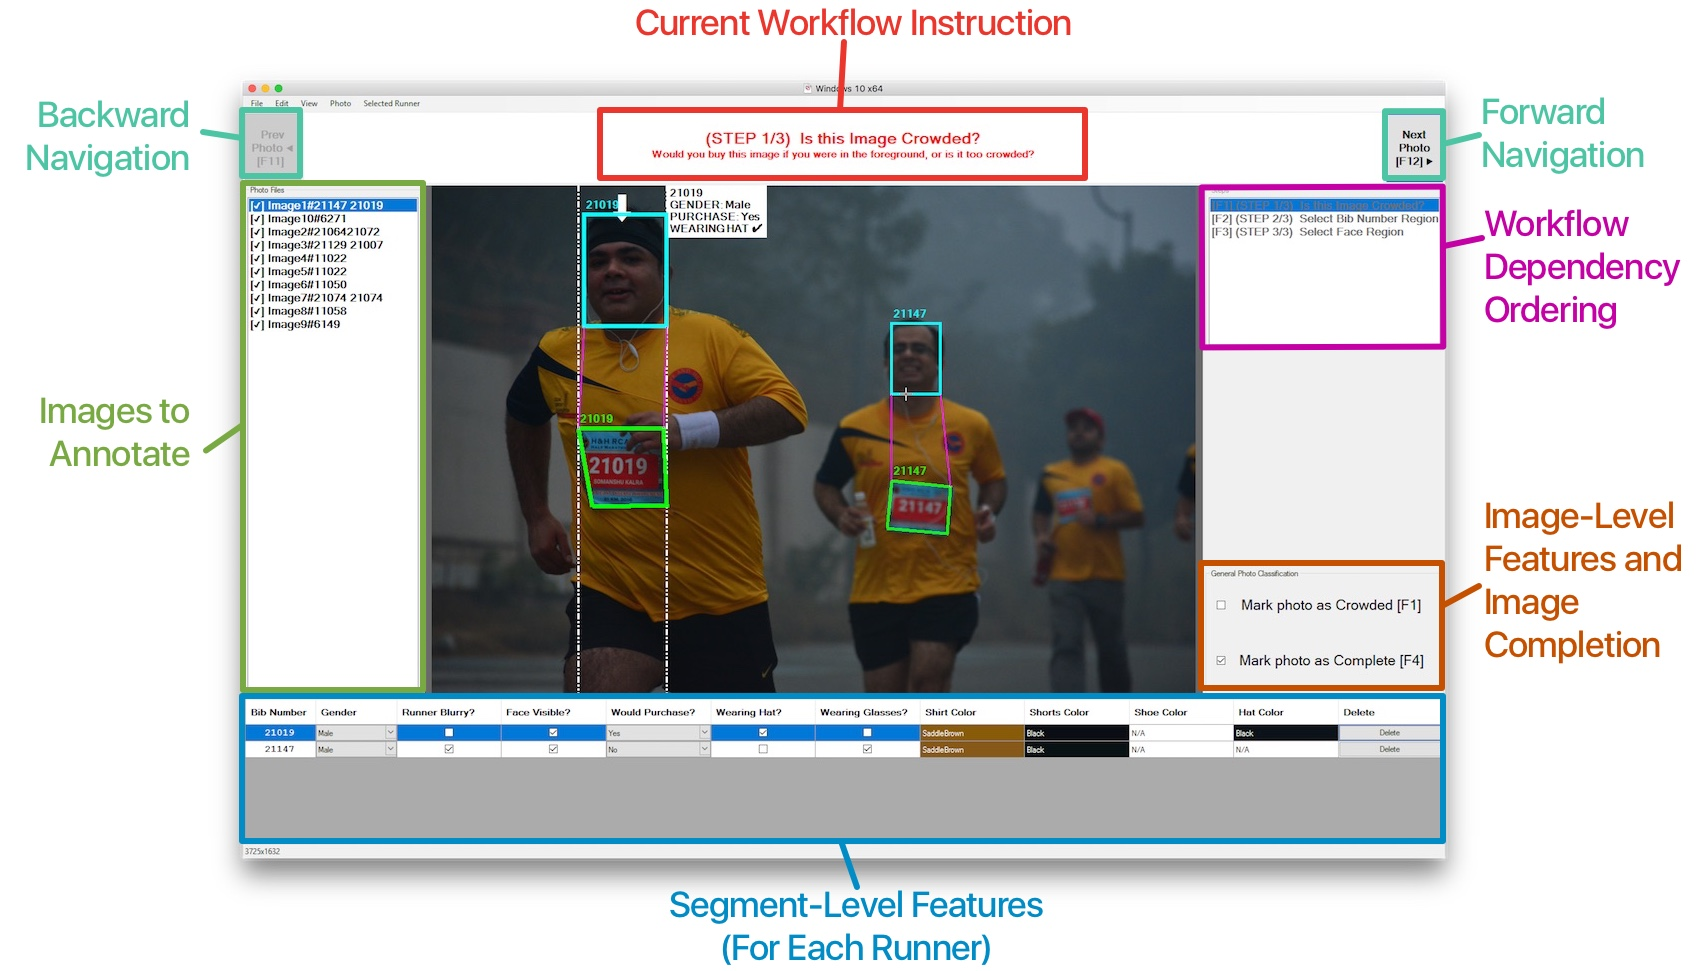
\includegraphics[width=\textwidth]{images/dataset/argus/argus_ui}
  \caption[An overview of the Argus user interface]{An overview of the Argus user interface.}
  \label{fig:dataset:argus:overview}
\end{figure}

\begin{figure}
  \centering
  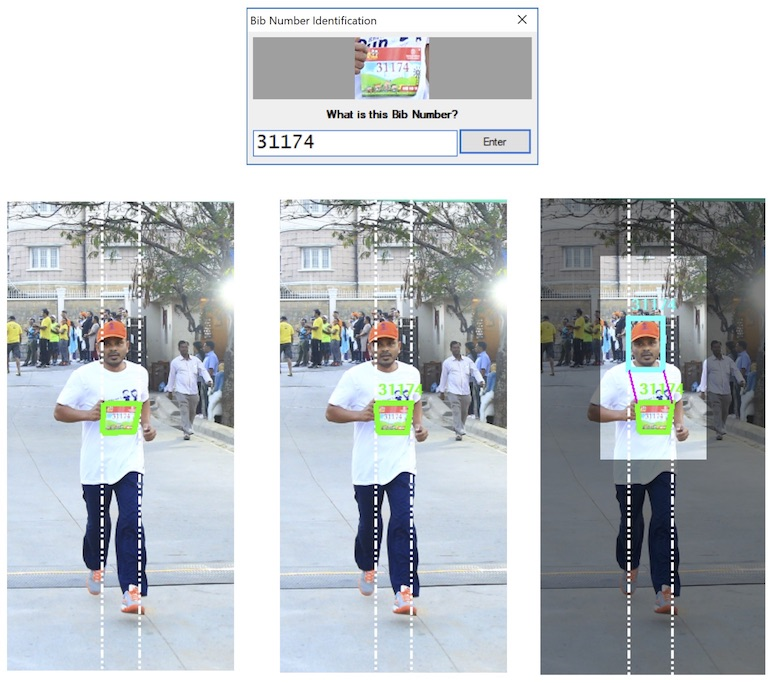
\includegraphics[width=\textwidth]{images/dataset/argus/argus_entry}
  \caption[Bib and Face feature annotation with Argus]{$Bib$ and $Face$ segment-level feature annotation. Users click four times around the bib to mark up the $BibSheet$ region (left). A dialog asks the user to enter the $\gls{rbn}$ label (top). The \gls{rbn} is annotated on the image (middle) and users can progress to drag-and-drop around the $Face$ region within the restrictions set (see \cref{sec:dataset:architecture:metamodel}). Note the dependency ordering is present.}
  \label{fig:dataset:argus:bib_and_face}
\end{figure}

\begin{figure}
  \hspace{\fill}
  \begin{subfigure}[b]{0.45\textwidth}
    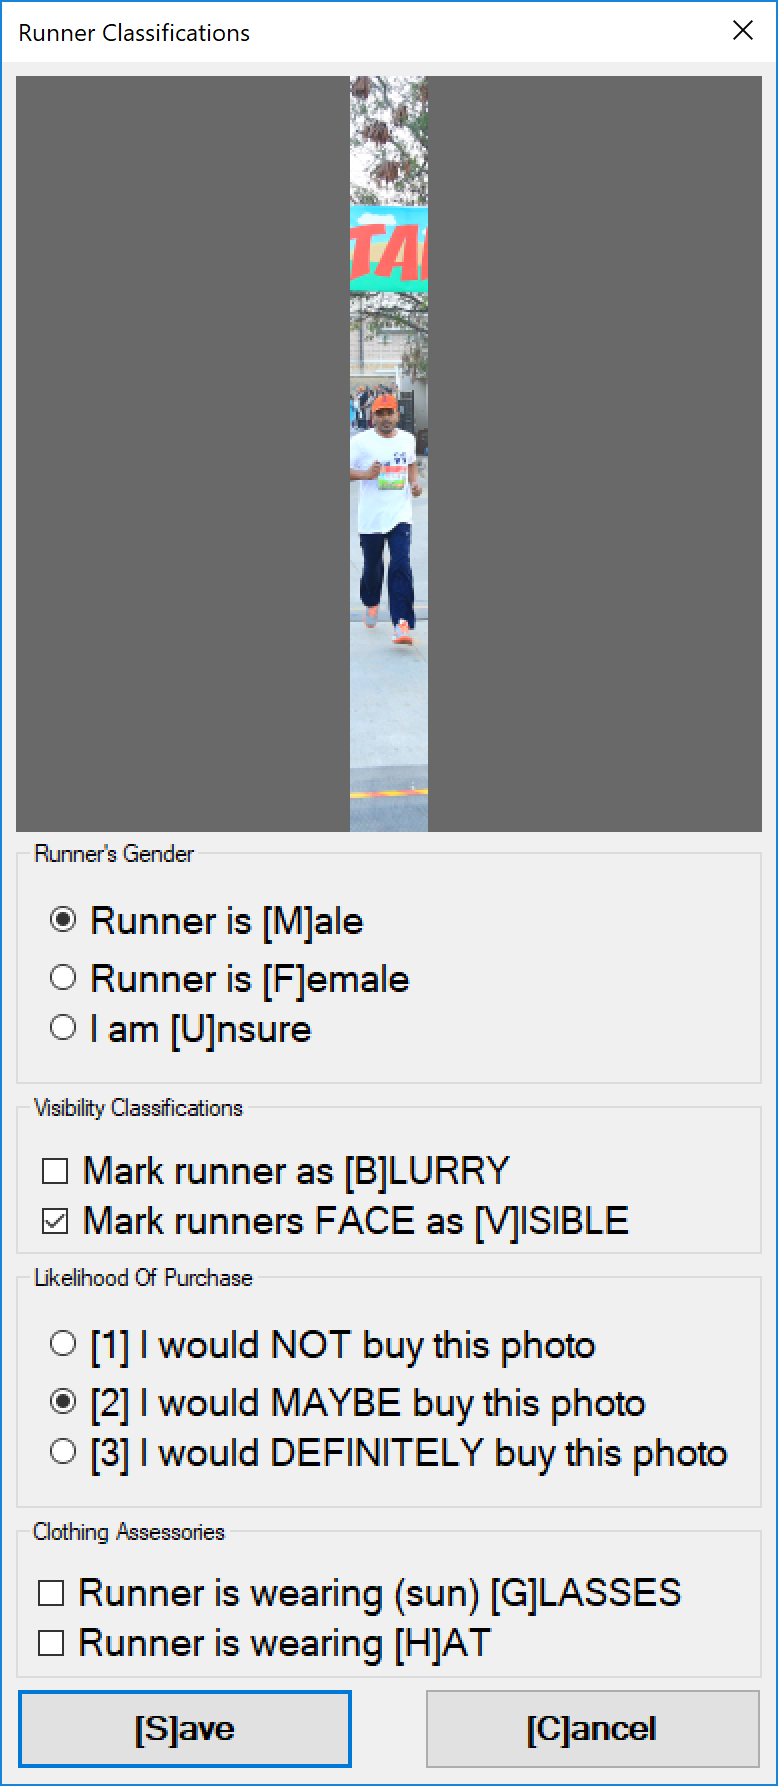
\includegraphics[width=\textwidth]{images/dataset/argus/argus_prom_entry}
  \end{subfigure}
  \hspace{\fill}
  \begin{subfigure}[b]{0.45\textwidth}
    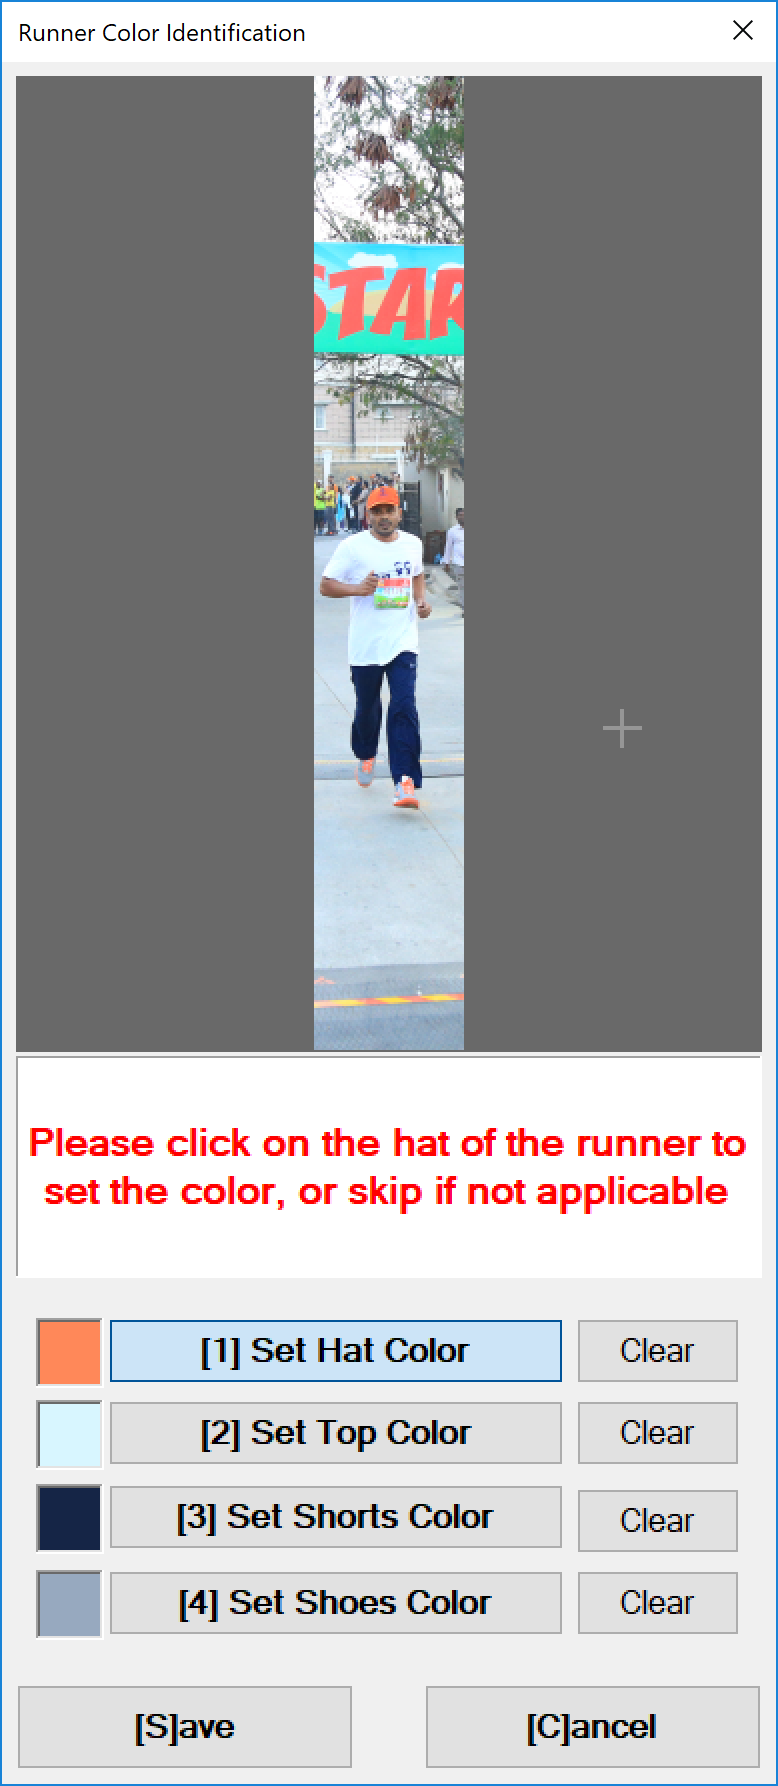
\includegraphics[width=\textwidth]{images/dataset/argus/argus_color_entry}
  \end{subfigure}
  \hspace{\fill}
  \caption[Prominence and Colour feature annotation with Argus]{Annotation for the $Prominence$ and $Colour$ segment-level features.}
  \label{fig:dataset:argus:prom_and_col}
\end{figure}

We deployed Argus to data taggers remotely using the ClickOnce Deployment\footnoteurl{https://msdn.microsoft.com/en-us/library/t71a733d.aspx}{11 August 2017} strategy.
\section{System Evaluation}

We evaluated our implementation for throughput, biases on the \glsx{lop}, and the general quality of the annotations made by data taggers. We break this evaluation under various metrics in the following sections.

\subsection{Annotation Throughput}
\label{sec:dataset:argus:metrics}

While Argus is running, we gather a number of metrics to determine what throughput is achievable in our 803 images, presented in  \cref{fig:dataset:argus:metrics:throughput}. We measure throughput as either image-level of segment-level features. A single image usually takes less than a minute to markup, and the longest feature to markup is the prominence and face features, especially as we gather most annotations here. These statistics are useful for productivity analysis on how long a given dataset may take to markup using Argus.

\begin{figure}[h]
  \begin{subfigure}[b]{\textwidth}
    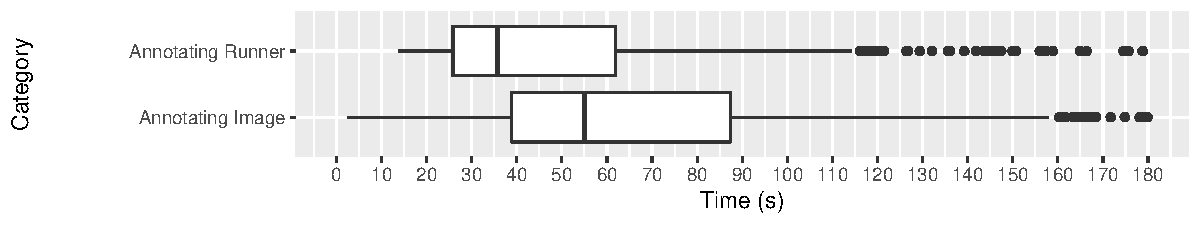
\includegraphics[width=\textwidth]{images/dataset/argus/photo_box_plots}
    \caption{Overall timing per image.}   
  \end{subfigure}
  \smallskip
  \\
  \begin{subfigure}[b]{\textwidth}
    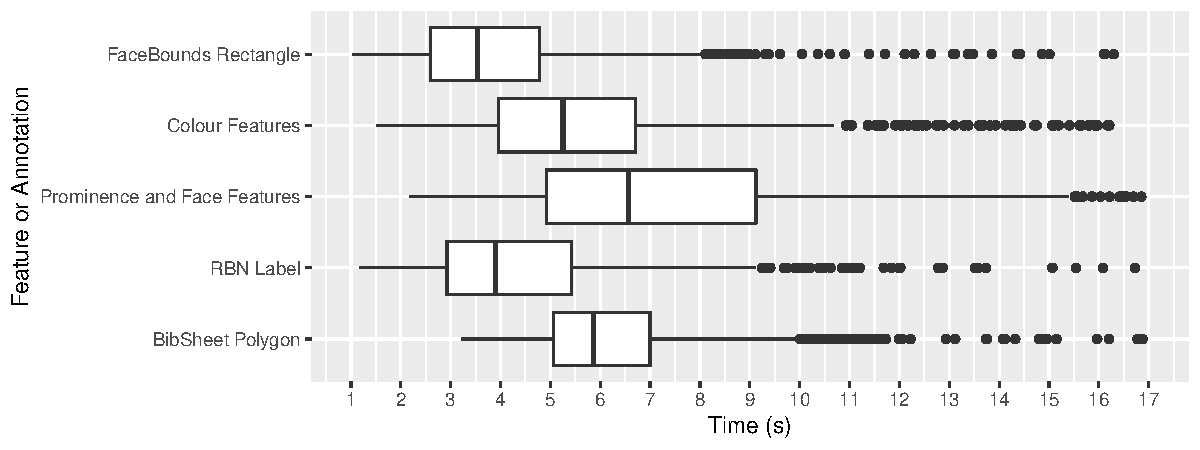
\includegraphics[width=\textwidth]{images/dataset/argus/feature_box_plots}
    \caption{Segment-level features and annotations marked up.}   
  \end{subfigure}
  \caption[Throughput of images using Argus]{Throughput of 803 images using Argus.}
  \label{fig:dataset:argus:metrics:throughput}
\end{figure}

Another metric gathered were the number of mistakes made during annotation. We define `mistake' as a rule violation, \gls{ui} violation, or poor data entry. As shown in \cref{tab:dataset:argus:metrics:mistakes}, adding construction rules is useful for our metamodel, as discovered during deployment trials of Argus. We needed to add the $FaceBounds$ restriction (\cref{fig:dataset:issues_with_tagging}), which was then violated a further 130 times during our annotation. \gls{ui} restrictions automatically built into Argus also proved useful. These restrictions  prevented users from dragging-and-dropping from bottom-right to top-left (inverse rectangle)\footnote{Although, it would have been possible to automatically swap the $x_{1}$ and $y_{1}$ with $x_{2}$ and $y_{2}$ within Argus.} or checking if a polygon was being dragged-and-dropped instead of clicked (and vice versa for rectangles).

\begin{table}[p]
  \centering
  \caption[Mistakes using Argus]{Frequencies of mistakes made during the annotation process. These are separated into construction rule violations, \gls{ui} violations, and poor data entry.}
  \label{tab:dataset:argus:metrics:mistakes}
  \begin{tabular}{@{}ll@{}}
    \toprule
    \textbf{Statistic}                                & \textbf{Frequency} \\ \midrule
    Marked as complete when $Face$ region not tagged  & 20                 \\
    Selected outside $FaceBounds$ restriction         & 130                \\
    Selected $FaceBounds$ below $BibSheet$            & 7                  \\
    \midrule
    Drag-and-drop inversely for $FaceBounds$          & 4                  \\
    Drag-and-drop made for $BibSheet$ polygon         & 73                 \\
    Clicked instead of drag-and-drop for $FaceBounds$ & 45                 \\
    \midrule
    Undos made                                        & 70                 \\
    Deleted runner annotation                         & 46                 \\ \bottomrule
  \end{tabular}
\end{table}

\subsection{Annotation Likelihood of Purchase Bias}

Upon inspection of our \glsx{lop} metrics, we found that, of all runner's that were annotated (1,031), 77.1\% were marked with a \gls{lop} of \textsc{yes}, 10.7\% were marked as \textsc{maybe} and 12.2\% were marked as \textsc{no}. These values are important for prominence ranking training, as we we know there are far more prominent runners (with a higher \gls{lop}) to train an \gls{ai} model. Furthermore, we want to reduce as many \textsc{maybe} \gls{lop} values as possible as these annotations are discarded in prominence training to reduce impartial bias when training a \gls{nn}---and as shown our dataset was annotated with the \textsc{maybe} values at a minimum. Augmentation (\cref{sec:dataset:postprocessing:augmentation}) is required to increase the number of \textsc{no} training samples.

\subsection{Annotation Quality Evaluation}
\label{sec:dataset:argus:quality_eval}

We took a subset of 260 randomly selected images  (approximately one third of the entire dataset) tagged from the data tagging team and assessed the photos for quality assurance. Here, we inspected photos on three tiers: `Good', `Okay', and `Bad' quality. We deemed photos as `Good' if there were no flaws at all with the tagging, `Okay' if there were minor errors made that we can compensate with, and `Bad' if there are significant flaws with the tagging that would affect the \gls{ai} model. Refer to \cref{fig:dataset:argus:qualituy_tiers} for samples of these images.

\begin{figure}[p]
  \hspace{\fill}
  \begin{subfigure}[b]{0.30\textwidth}
    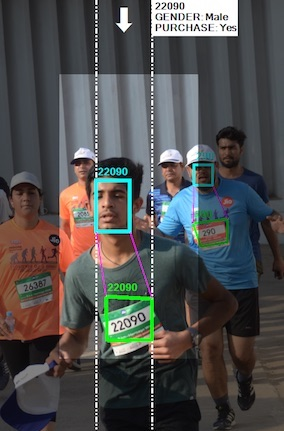
\includegraphics[width=\textwidth]{images/dataset/argus/quality_tagging_bad_polygons}
    \caption{A `Bad' annotation}
    \label{fig:dataset:argus:qualituy_tiers:bad_polygons}
  \end{subfigure}
  \hspace{\fill}
  \begin{subfigure}[b]{0.30\textwidth}
    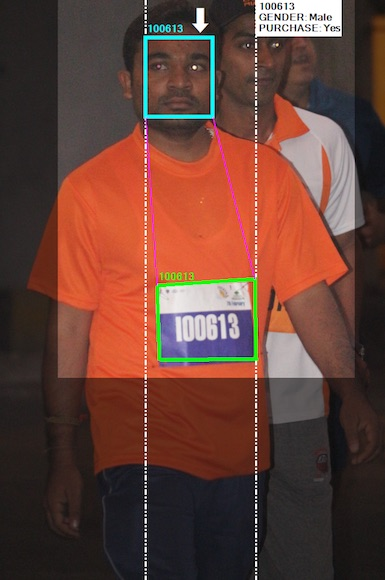
\includegraphics[width=\textwidth]{images/dataset/argus/quality_tagging_bad_invalid_rbn}
    \caption{A `Bad' annotation}
    \label{fig:dataset:argus:qualituy_tiers:bad_invalid_rbn}
  \end{subfigure}
  \hspace{\fill}
  \begin{subfigure}[b]{0.30\textwidth}
    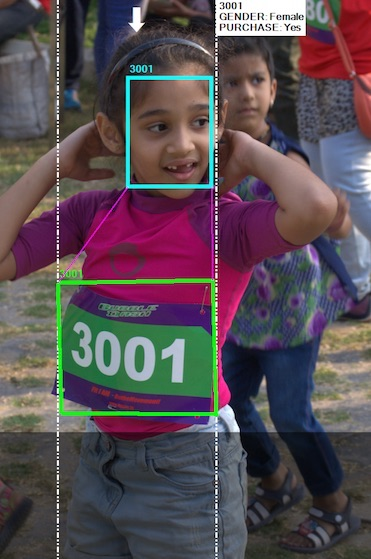
\includegraphics[width=\textwidth]{images/dataset/argus/quality_tagging_okay}
    \caption{An `Okay' annotation}
      \label{fig:dataset:argus:qualituy_tiers:okay}
  \end{subfigure}
  \hspace{\fill}
  \caption[Quality assurance using Argus]{`Okay' and `Bad' quality tagging tiers.}
  \label{fig:dataset:argus:qualituy_tiers}
\end{figure}

In \cref{fig:dataset:argus:qualituy_tiers:okay}, we see that the $FaceBounds$ annotation is too small around the runner's head, and that the $BibSheet$ polygon has been marked as a square, rather than directly around the four corners of the bib sheet. This is considered `Okay' as we are able to compensate with the extra padding around the $BibSheet$, and the $FaceBounds$ could have padding to extend the area. In \cref{fig:dataset:argus:qualituy_tiers:bad_polygons,fig:dataset:argus:qualituy_tiers:bad_invalid_rbn}, however, we are given completely incorrect information. In the former, the $BibSheet$ polygon is not at all reflective of the actual sheet, including part of the runner's shirt in the annotation, and the $FaceRegion$ is too small unless significant padding is added. In the latter, the $\gls{rbn}$ has been annotated with the value \texttt{\textbf{1}00613}, confusing the first character as numeric when it is alphabetic (\texttt{\textbf{I}00613}). These instances show significant fallbacks to quality that may hinder training the \gls{nn}.

In our sample set, we also evaluated whether the number of runner's in an overall photo has a negative impact on the annotation quality (\cref{fig:dataset:argus:quality_of_tagging_count}), as well as how long taggers spend on annotating photos (\cref{fig:dataset:argus:quality_of_tagging_time}). Upon analysis, we can see that most runners are well-annotated---only in images containing one runner where there are more `Bad' annotations than `Okay' ones, and generally `Okay' and `Good' outcomes are largely consistent regardless of runner count. Therefore, likelihood of time spent on annotations is `Good', and `Bad' marking distribution is more biased towards short evaluation times where there are few runners in the image. \cref{fig:dataset:argus:quality_of_tagging_time} confirms our hypothesis where, we can see, the longer the annotator spend time tagging, the better the quality of our data is: a median of 48 seconds is improved to 52 seconds between `Bad' and `Okay', and this jumps to a median of 55 seconds for `Good'. Therefore a difference in 7 seconds spend on tagging a photo shows a significant improvement on the quality of the tagging.

\clearpage

\begin{figure}[p]
  \centering
  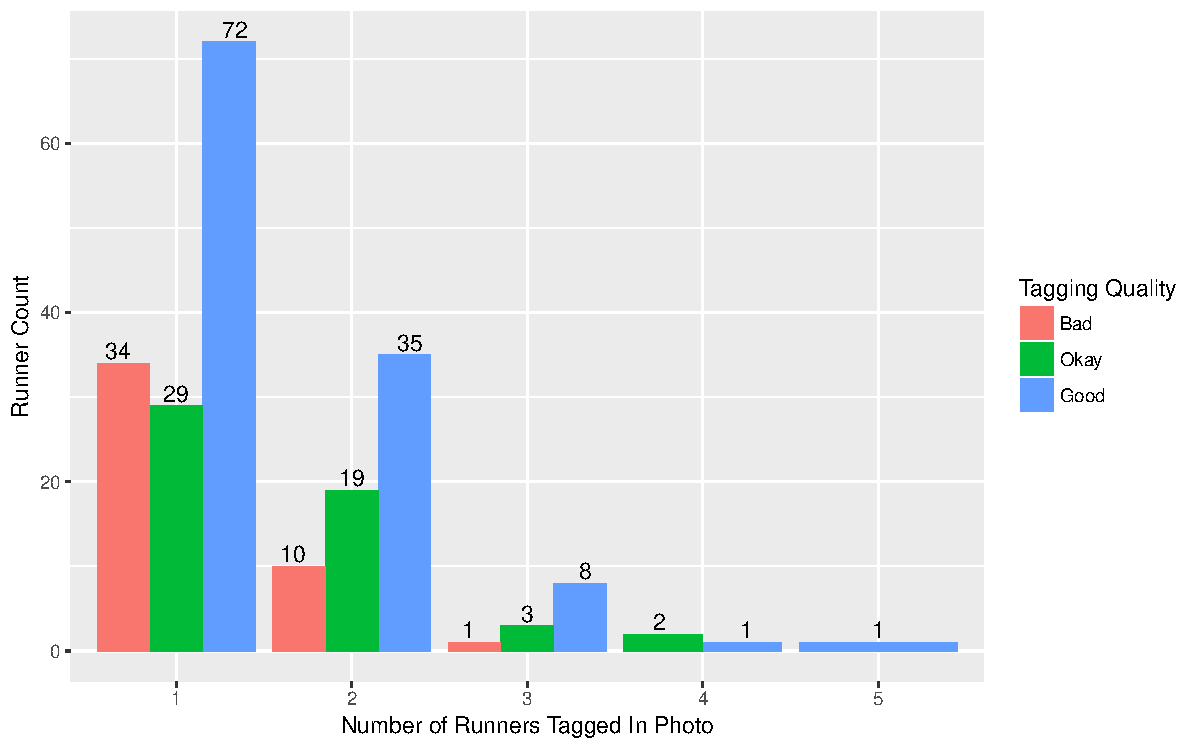
\includegraphics[width=0.9\textwidth]{images/dataset/argus/quality_of_tagging_count}
  \caption[Quality of tagging related the number of runners per photo]{The quality of tagging against the number of runners per photo.}
  \label{fig:dataset:argus:quality_of_tagging_count}
\end{figure}

\begin{figure}[p]
  \centering
  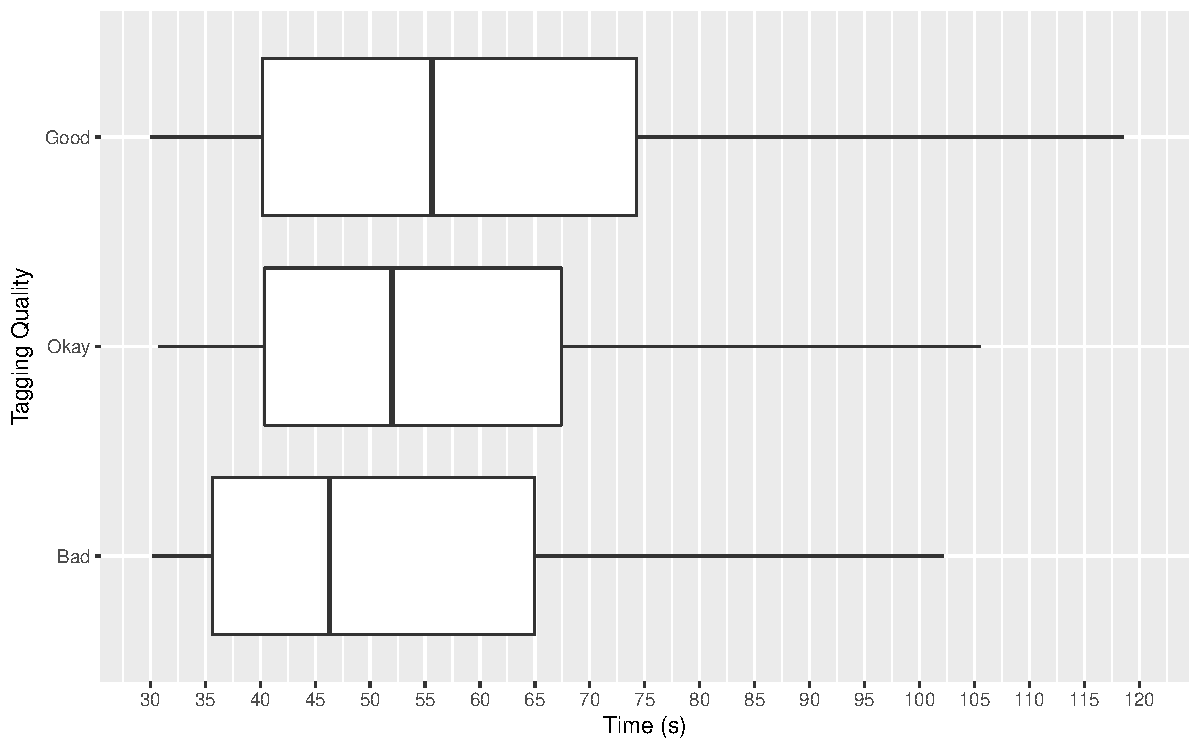
\includegraphics[width=0.9\textwidth]{images/dataset/argus/quality_of_tagging_time}
  \caption[Quality of tagging and seconds evaluating the photo]{Quality of tagging against the time spent evaluating the photo.}
  \label{fig:dataset:argus:quality_of_tagging_time}
\end{figure}

\clearpage
\section{Comparative Annotation Tools}
\label{sec:dataset:architecture_evaluation:tools}

In this section, we describe comparative annotation tools and services used to annotate similar datasets, and compare such tools with Argus.

\subsection{LabelMe} 

LabelMe\footnoteurl{http://labelme.csail.mit.edu/}{17 August 2017} (\cref{fig:dataset:architecture_evaluation:tools:label_me}), developed by \citet{Russell:2008wm}, is a web-based application that requires annotators to set up the web service on their own system. It has been successfully used to markup the large \gls{sun} dataset by novice users, though the developers note a number of reflective fallbacks and potential difficulties using the tool \citep{DBLP:journals/corr/abs-1210-3448}. LabelMe does not contain a specific instructional workflow, unlike Argus, and therefore annotators are allowed to selectively choose whichever objects to annotate\footnote{Instructions are potentially vague: ``Use your mouse to click around the boundary of \textit{some} objects''.}. This makes the resulting dataset largely incomplete as (potentially) not all objects in each image are fully annotated. Additionally, there is no restriction to what types of objects are annotated in the image, as any text can be used to describe an object (rather from a hierarchical category, such as in \citep{Lin:2014vma}).

\begin{figure}[h]
  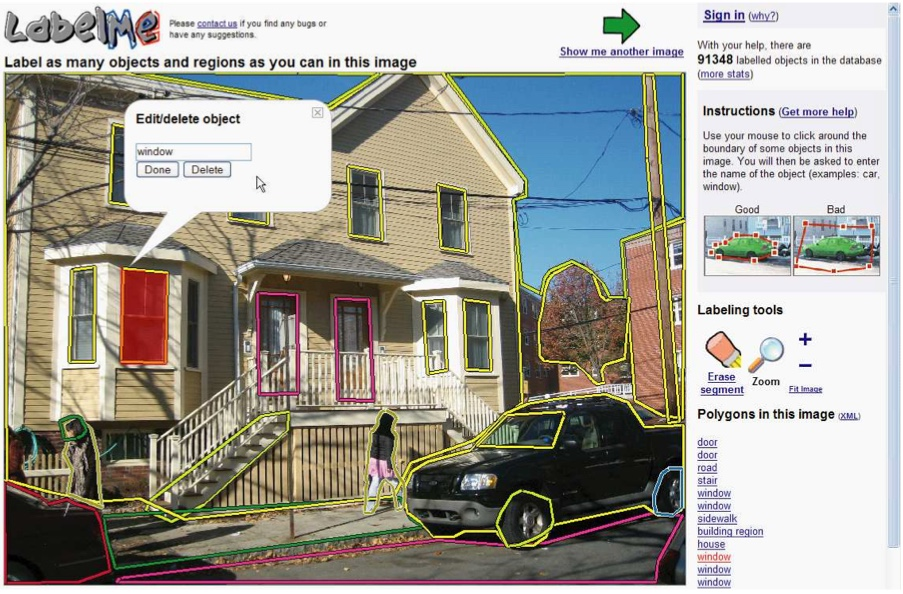
\includegraphics[width=\textwidth]{images/dataset/tools/label_me}
  \caption[The LabelMe user interface]{The LabelMe user interface \citep{Russell:2008wm}.}
  \label{fig:dataset:architecture_evaluation:tools:label_me}
\end{figure}

\subsection{Annotation and Performance Evaluation Platform} 

\citet{Karatzas:2014bt} introduced the \glsac{cvc} \gls{apep}\footnoteurl{http://www.cvc.uab.es/apep/}{17 August 2017}, made popular for use using the \gls{icdar} 2011--2015 Robust Reading Competitions. Unlike our system, users can edit the per-pixel boundaries using a `flood-fill' or `magic-select' markup tool (with an adjustable tolerance), followed by a skeletonisation of the boundaries filled. This speeds up selection of specific text areas (\cref{fig:dataset:architecture_evaluation:tools:apep}). While we did not incorporate a feature into Argus, a potential future version would benefit using such an annotation tool for a polygon, rather than clicking $n_{vertices}$ times if the vertices count is unknown. This could also be encoded using \gls{rle} as suggested from the \gls{coco} format in \cref{sec:dataset:architecture_evaluation}. Additionally, users are able to zoom in to get finer accuracies at the pixel level.


\begin{figure}[h]
  \centering
  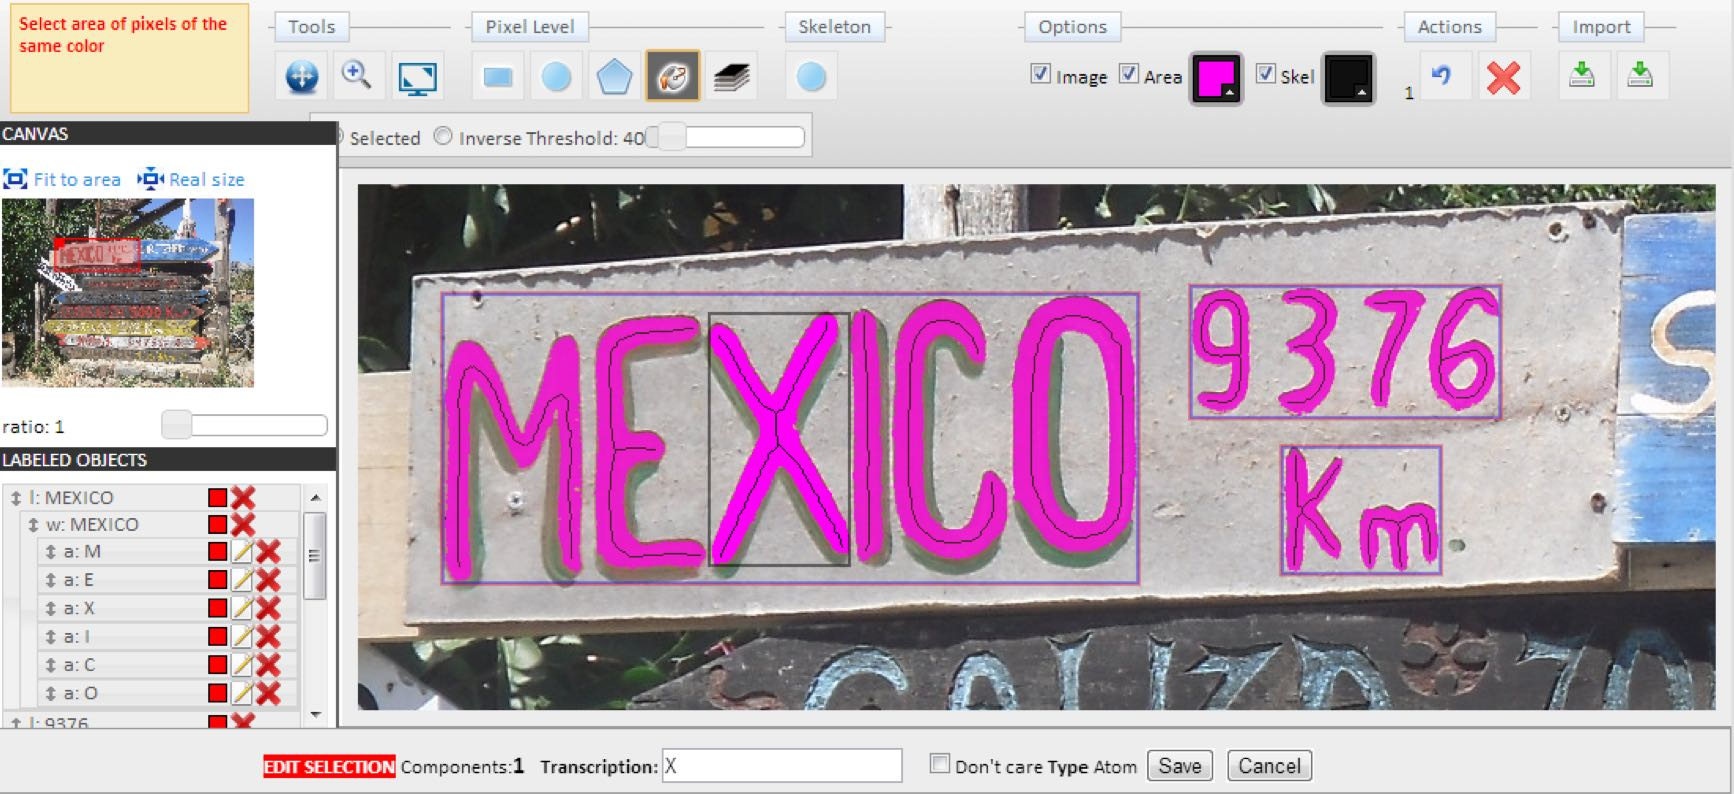
\includegraphics[width=0.9\textwidth]{images/dataset/tools/apep}
  \caption[The APEP user interface]{The APEP ground truth annotation tool, showing a hierachy of textual content and defined text parts (flood-filled areas and skeletons) \cite{Karatzas:2014bt}.}
  \label{fig:dataset:architecture_evaluation:tools:apep}
\end{figure}

% Robust Reading Competition by the Computer Vision Centre: http://www.cvc.uab.es/apep/images/DAS2014_Toolbox.pdf
% ICDAR12-15 which uses CVC Annotation and Performance Evaluation Platform (APEP) \cite{Karatzas:2015tj}

\vspace{-2em}
\subsection{Amazon Mechanical Turk}

\gls{amt}\footnoteurl{https://www.mturk.com/mturk/welcome}{11 August 2017} provides \gls{saas} that does not require downloading or setting up (typically laborious for annotators). Annotation is achieved in the form of customised \glspl{hit}, using a custom-built interface. Recently, this is typically the most popular choice of annotation outsourcing \citep{Lin:2014vma,Veit:2016vj,Chen:2015ur,JiaDeng:2009dl,Netzer:2011to} due to flexibility in developing customised interfaces for the task at hand. The benefits of ensuring a user-friendly crowdsourcing annotation system are presented by \citet{Matera:2014wq}. \citet{Sorokin:2008uk} discuss the utility of using \gls{amt} for annotation. The primary downside is that most interfaces need to be created from scratch, which can typically be laborious.

\subsection{VATIC}

\glsdisp{vatic}{VATIC (the \glsdesc{vatic})} is a a free web-based tool (\cref{fig:dataset:architecture_evaluation:tools:vatic}) developed by \citet{springerlink:10.1007/s11263-012-0564-1}, running on \gls{amt}. We note this tool specifically for the use of annotating video stills within an image: its intended purpose is for the sole use of object tracking in videos. There are only three annotations per object: the object name, the object is out of view, and the object is obstructed. It is useful in that not all frames have to be individually annotated, as the tool uses object tracking to estimate the movement between every 2-3 seconds. This may be useful to incorporate into future works of Argus. 

\begin{figure}[h]
  \centering
  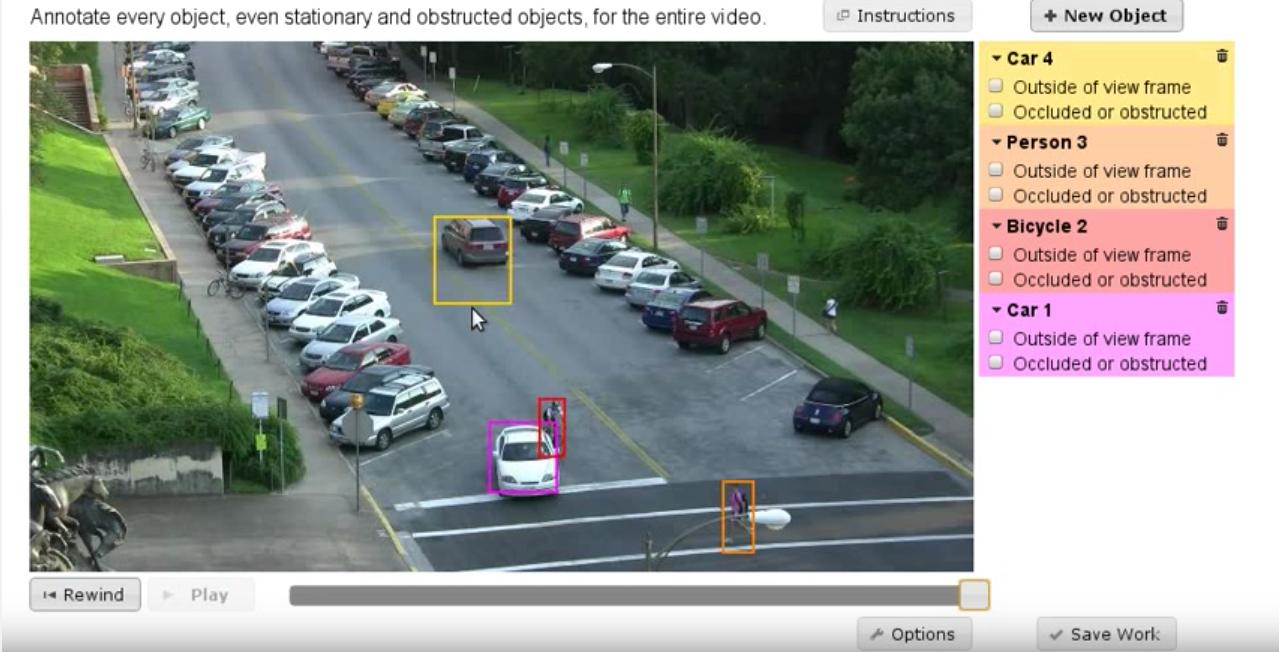
\includegraphics[width=0.9\textwidth]{images/dataset/tools/vatic}
  \caption[The VATIC web-based user interface]{The \gls{vatic} web-based user interface. Sourced from \url{https://github.com/cvondrick/vatic}. (Last viewed 11 August, 2017.)}
  \label{fig:dataset:architecture_evaluation:tools:vatic}
\end{figure}

% - http://carlvondrick.com/vatic/ -> amazon turk
%% Only for object tracking in videos
%% No annotations, only two attributes per feature: (outside view frame or obfuscated)
%% Cannot label each feature, it's Car 1, Car 2, Car 3... may be hard for long videos. 
%% Useful in that you do not need to process every frame
%% PAPER: Utility data annotation with amazon mechanical turk

\vspace{-2em}
\subsection{ScaleAPI}

ScaleAPI\footnoteurl{http://www.scaleapi.com}{11 August 2017} is a recent \gls{saas} that provides a web-based \gls{api} to return human-marked annotation in realtime. Various boundary annotations can be made on an image. \cref{lst:dataset:evaluation:scaleapi:req,lst:dataset:evaluation:scaleapi:res} show the request and response for a simple instruction to draw bounding boxes around all pedestrians and cars in the image\footnoteurl{https://docs.scaleapi.com/?shell\#bounding-box-annotation}{17 August 2017}. Additionally, object segmentation (on a per-pixel basis) is provided. While there are no need for workflows in a single request (as multiple requests can be made for multiple workflow steps), instructions to annotators are provided on a per-request basis. This said, a consistent annotator between requests is not guaranteed and this may have an impact on varying annotator quality.

\begin{lstlisting}[language=CURL, label=lst:dataset:evaluation:scaleapi:req, caption={[Sample ScaleAPI request] A sample ScaleAPI HTTP request made using cURL\footnotemark.}]
curl "https://api.scaleapi.com/v1/task/annotation" \
  -u "SCALE_API_KEY:" \
  -d callback_url="http://www.example.com/callback" \
  -d instruction="Draw a box around each **car** and **pedestrian**." \
  -d attachment_type=image \
  -d attachment="http://i.imgur.com/XOJbalC.jpg" \
  -d objects_to_annotate="car" \
  -d objects_to_annotate="pedestrian" \
  -d with_labels=true \
  -d min_width="30" \
  -d min_height="30"  
\end{lstlisting}
\footnotetext{\url{https://curl.haxx.se/} last accessed 17 August 2017.}

\begin{lstlisting}[language=JSON, label=lst:dataset:evaluation:scaleapi:res, caption={[Sample ScaleAPI response] Sample \glsac{json} response from the request made in \cref{lst:dataset:evaluation:scaleapi:req}.}]
{
  "task_id": "5774cc78b01249ab09f089dd",
  "created_at": "2016-9-03T07:38:32.368Z",
  "callback_url": "http://www.example.com/callback",
  "type": "annotation",
  "status": "pending",
  "instruction": "Draw a box around each **car** and **pedestrian**",
  "urgency": "day",
  "params": {
    "with_labels": true,
    "min_width": 30,
    "min_height": 30,
    "objects_to_annotate": [
      "car",
      "pedestrian"
    ],
    "attachment_type": "image",
    "attachment": "http://i.imgur.com/XOJbalC.jpg"
  },
  "metadata": {}
}
\end{lstlisting}


\section{Summary}

This chapter presents Argus, the implementation of our metamodel shown in \cref{ch:dataset}. We present the overall \gls{ui} in Argus, and evaluate it against three key metrics: throughput, bias and quality. We also present comparative annotation tools that we assess against Argus to find specific overlaps between both.

\bigskip

\noindent
The primary contributions of this chapter are:

\begin{itemize}
  \item an open-source dataset tagging system for \gls{rbn} and prominence extraction, \textit{Argus}
  \item an assessment of data tagger performance and throughput for specific phases in marathon-racing dataset tagging, and
  \item a methodology for quality assessment of annotations made in a dataset.
\end{itemize}

\noindent
Minor contributions in this chapter include:

\begin{itemize}
  \item a comparison of our proposed system against existing comparative annotation tools.
\end{itemize}